\documentclass[a4paper]{article}

\usepackage[utf8]{inputenc}

\usepackage{fullpage}
\usepackage{amsfonts}
\usepackage{amsmath}
\usepackage{amssymb}
\usepackage{bbold}
\usepackage{array}

\usepackage{graphicx}

\setlength\parindent{0pt}

\title{CR11 --- Mathematical methods for image synthesis} 
\author{Simon Mauras}
\date{December 20\textsuperscript{th} 2017}

\graphicspath{{../Slides/}}

\begin{document}
  
  \maketitle
  
  \section{Article: Stable Region Correspondences}

  \subsection{Motivations}

  The article I decided to study is "Stable Region Correspondences Between Non-Isometric Shapes". Authors are V. Ganapathi-Subramanian, B.Thibert, M. Ovsjanikov and L. Guibas. It has been published in \textit{Computer Graphics Forum}. Vol. 35. No. 5. 2016.
  
  \bigskip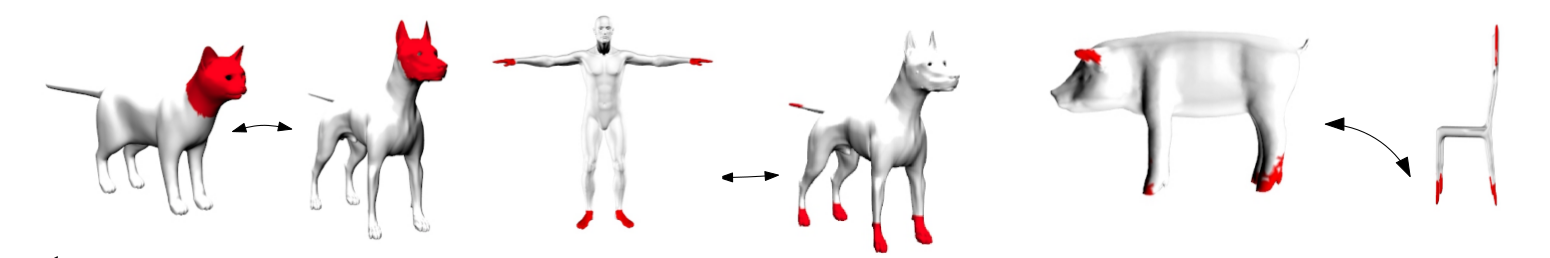
\includegraphics[width=\textwidth]{article/intro.png}
  
  The goal of this article is to find similar regions between two shape. The case where both shapes are isometric is easier, as there is a one to one map from between the set of vertices. Here the approach is to use classical feature functions (\text{e.g.} Gaussian curvature) to achieve good and stable results.

  \subsection{Affinity Matrix}

  We are given two shapes as triangulated meshes. Their vertex sets are $S^{(1)} = \{p_1, \dots, p_{d_1}\}$ and $S^{(2)} = \{q_1, \dots, q_{d_2}\}$. We define two functions $f^{(1)}$ and $f^{(2)}$ implementing the same feature.
  \[f^{(1)} : S^{(1)} \mapsto \mathbb R \quad\text{and}\quad f^{(2)} : S^{(2)} \mapsto \mathbb R\]
  
  In the image below (from the article), are ploted two features : a multiscale mean curvature and a WKS signature.
  
  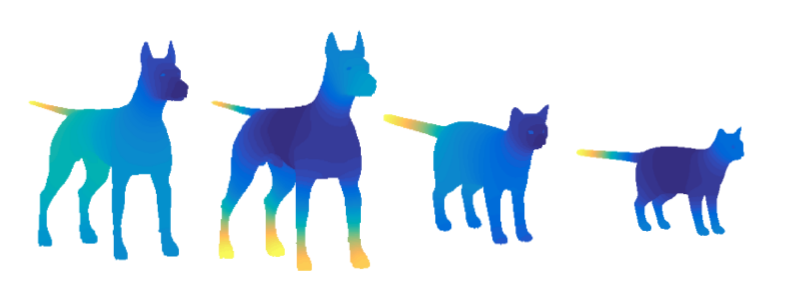
\includegraphics[width=\textwidth]{article/features.png}
  
  We can notice that even if values are different on the two shapes, the rank of a value is meaningfull. 
  
  \newpage
  
  We define to permutations $r^{(1)}$ and $r^{(2)}$ of $\mathfrak S_n$:
  \[r^{(1)}_i = j \;\text{ if }f^{(1)}(p_j)\text{ is the }i^{th}\text{ value in sorted order.}\]
  \[r^{(2)}_i = j \;\text{ if }f^{(2)}(q_j)\text{ is the }i^{th}\text{ value in sorted order.}\]
  
  \medskip Let $K$ be an integer that divides $d_1$ and $d_2$. For $1 \leq k \leq K$:
  \[C_k^{(1)} = \left\{r^{(1)}_i \;\middle|\; (k-1)\frac{d_1}{K} \lneq i \leq k\frac{d_1}{K} \right\}\]
  \[C_k^{(2)} = \left\{r^{(2)}_i \;\middle|\; (k-1)\frac{d_2}{K} \lneq i \leq k\frac{d_2}{K} \right\}\]

The affinity matrix of feature $(f^{(1)}, f^{(2)})$ can be defined as follow.
\[W = \sum_{k=1}^K \mathbb 1_{C^{(2)}_k} \cdot \mathbb 1_{C^{(1)}_k}^T = \underbrace{\left(\begin{array}{ccc|ccc|ccc}
1 & \dots & 1 & && & && \\
\vdots & & \vdots & &(0)& & &(0)& \\
1 & \dots & 1 & && & && \\\hline
&& & 1 & \dots & 1 & &&\\
&(0)& & \vdots & & \vdots & &(0)&\\
&& & 1 & \dots & 1 & &&\\\hline
&& & && & 1 & \dots & 1\\
&(0)& & &(0)& & \vdots && \vdots\\
&& & && & 1 & \dots & 1\\
\end{array}\right)}_{\displaystyle r^{(1)}_1 \; r^{(1)}_2 \hspace{4cm} r^{(1)}_{d_1}}\left\}\begin{array}{c}r^{(2)}_1\\r^{(2)}_2\\\\\\\\\\\\\\\\r^{(2)}_{d_2}\end{array}\right.\]
We can notice that coefficient $i,j$ of $W$ is equal to $1$ if $f^{(1)}(p_j)$ and $f^{(2)}(q_i)$ have similar ranks.

  \medskip If in a more general setting we consider $N$ different features, we can define the affinity matrix is the sum of each individual affinity matrix. Then we "normalize" the matrix by multiplying each coefficient by $K/(Nd_1d_2)$.
  
  \subsection{Stable pairs}

  To define stable pairs, and be able to compute similar regions between two shapes, some definitions are still required. Let $M$ be a matrix in $\mathcal M_n(\mathbb R)$.
  \begin{itemize}
    \item The norm $||M||$ is defined as the sum of the absolute value of all coefficients.
    \item The submatrix $M_{I,J}$ is obtained when keeping only lines $I \subseteq \{1, \dots, n\}$ and columns $J \subseteq \{1, \dots, n\}$.
  \end{itemize}
  
  We are now ready to define a stable pair $(\Omega^{(1)}, \Omega^{(2)})$ of size $(n,m)$. It is a subset $\Omega^{(1)} \times \Omega^{(2)} \subseteq S^{(1)} \times S^{(2)}$ with $|\Omega^{(1)}| = n$ and $|\Omega^{(2)}| = m$, such that $||W_{\Omega^{(2)}, \Omega^{(1)}}||$ is maximal.
  
  \medskip The existence of a global maximum is guaranted because there is only a finite number of submatrices. However we are interested in an efficient solution, that is going to be compute as the fixpoint of an operator (unfortunately non-linear).
  
  \medskip The procedure obtained is stable when adding i.i.d. random features. The image below gives example of the results that can be obtained.
  
  \bigskip 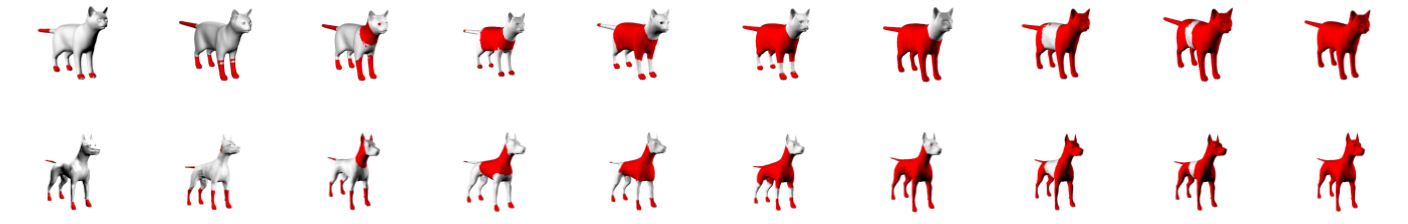
\includegraphics[width=\textwidth]{article/result.png}
  
  \newpage
  
  \section{Project: Poisson Image Editing}
  
  Our goal is to integrate an object (here a little girl) in an image (background). The figure below gives the naive solution for this problem. We can notice that the quality of the result is poor, the separation between the object and the background being visible.

  \bigskip
  \begin{tabular}{m{1.6cm}m{.6cm}m{1.6cm}m{.6cm}m{4.7cm}m{.6cm}m{4.7cm}}
    $\overbrace{\hspace{1.6cm}}^{\Omega}$ &&
    $\overbrace{\hspace{1.6cm}}^u$ &&
    $\overbrace{\hspace{4.7cm}}^v$ \\
    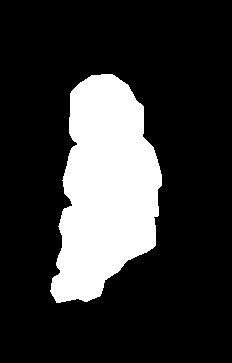
\includegraphics[scale=.2]{results_poisson/foreground-mask.png}
    & {\Huge$\times$} &
    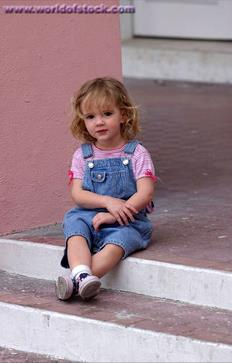
\includegraphics[scale=.2]{results_poisson/foreground.png}
    & {\Huge$+$} &
    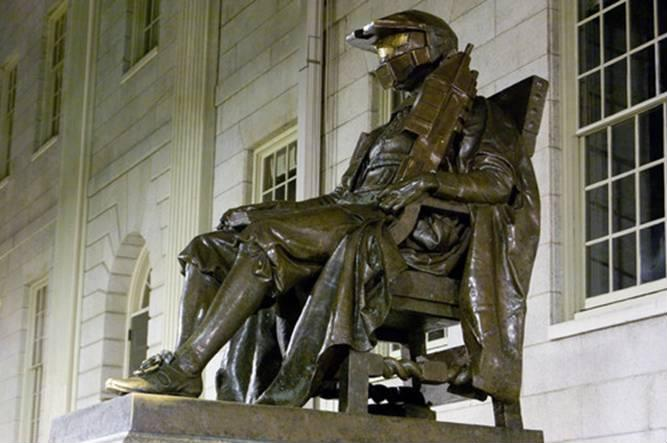
\includegraphics[scale=.2]{results_poisson/background.png}
    & {\Huge=} &
    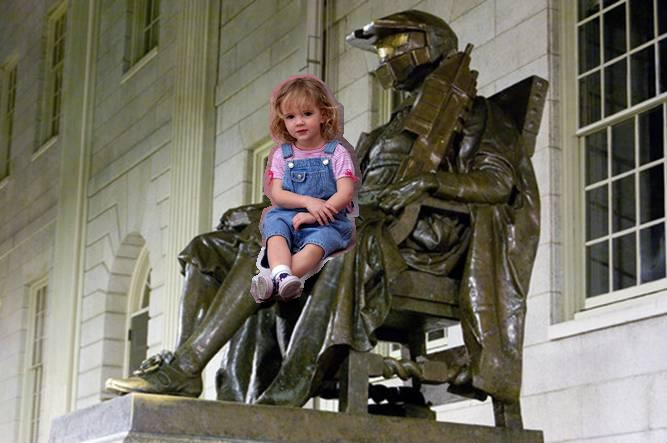
\includegraphics[scale=.2]{results_poisson/naive.png}
  \end{tabular}
  
  \medskip We have seen in class that the eye is more sensitive to color differences than absolute color values. A solution is the following, let $\tilde u$ such that $\tilde u = v$ on $\partial\Omega$ and $\mathcal L(\tilde u) = \int_\Omega |\nabla(\tilde u - u)|^2$ is minimized.
  
  \medskip This approach is developped in an article by Pérez, Gangnet and Blake: "Poisson image editing." in ACM Transactions on graphics (TOG). Vol. 22. No. 3. ACM, 2003.
  
  \iffalse
  \[\mathcal L[\tilde u + \delta u] - \mathcal L[\tilde u] = \int_{\Omega}|\nabla (\tilde u+ \delta u)|^2 - |\nabla u|^2\]
  We have $|\nabla (\tilde u+ \delta u)|^2 = |\nabla (\tilde u)|^2  + 2 \nabla (\tilde u) \cdot \nabla (\delta u) + |\nabla (\delta u)|^2$. We only keep first order terms.
  \[\mathcal L[\tilde u + \delta u] - \mathcal L[\tilde u] = \int_{\Omega} 2 \nabla (\tilde u) \cdot \nabla (\delta u) = \int_{\Omega} \nabla \cdot (\delta u \nabla \tilde u)\]
  \fi
  
  \subsection{Poisson equation}
  
  We can deduce a Poisson equation (using calculus of variation) from the previous minimization problem. 
  \[\nabla^2 \tilde u = 0 \quad\text{in }\Omega\]
  This equation can be discretized, to obtain a sparse linear system. We can solve it using the conjugate gradient method.
  
  \subsection{Implementation}
  
  I decided to implement this project in Python, as manipulating images is easier in this language. However performances are very far from those obtained using a low level language as C.
  
  \subsection{Results}
  
  Below are pictures after 1, 10, 100, 1000 and 10000 iterations of the conjugate gradient.
  
  \bigskip
  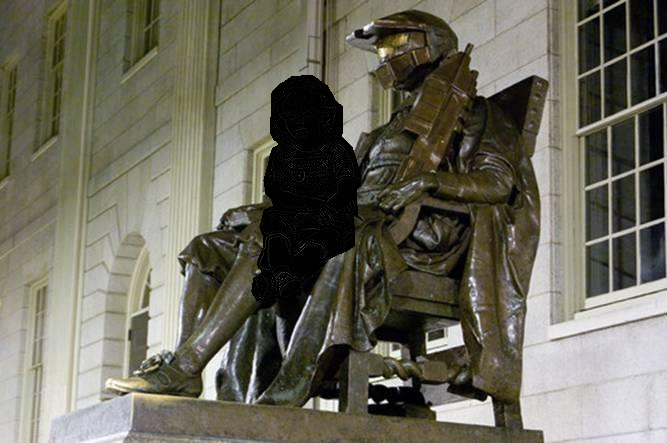
\includegraphics[width=.2\textwidth]{results_poisson/1.png}
  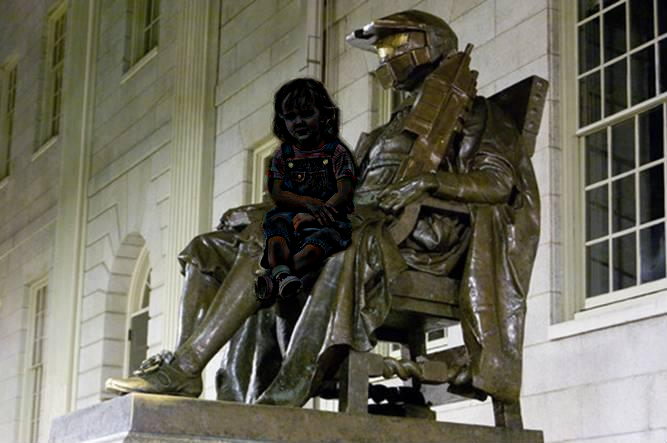
\includegraphics[width=.2\textwidth]{results_poisson/10.png}
  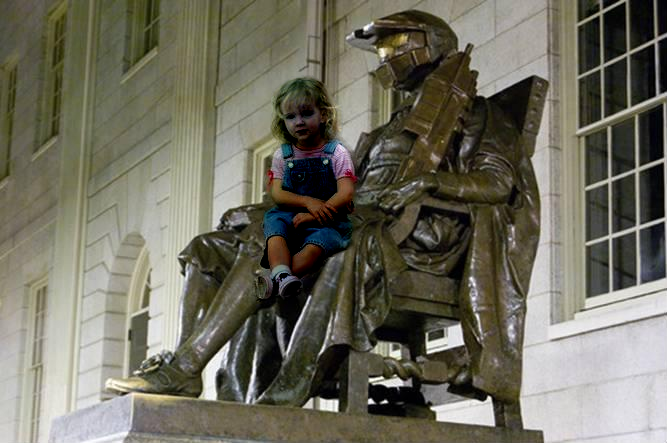
\includegraphics[width=.2\textwidth]{results_poisson/100.png}
  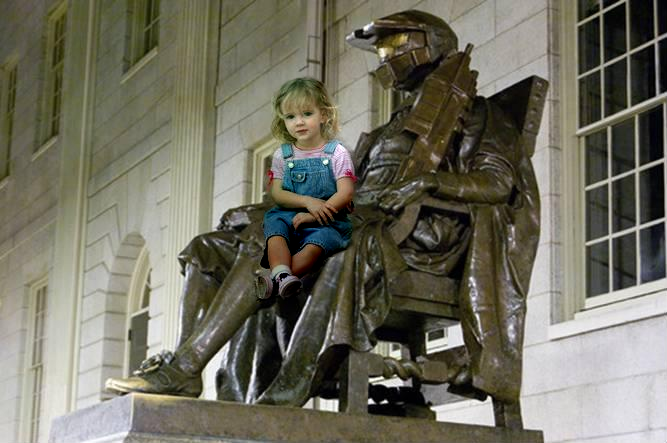
\includegraphics[width=.2\textwidth]{results_poisson/1000.png}
  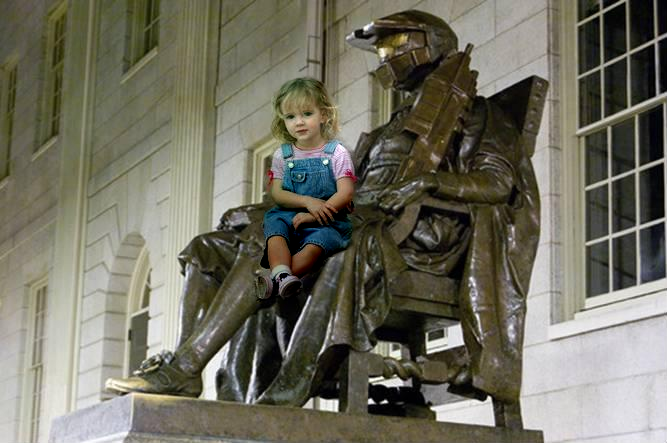
\includegraphics[width=.2\textwidth]{results_poisson/10000.png}
  
  \newpage
  
  \section{Project: Image Inpainting}
  
  The goal of this project is to remove a part of an image (\textit{e.g.} a person, ...) and replace it by a texture automaticaly generated from the rest of the image.
  
  \medskip The approach used is developped in the article "Image Analogies" from Hertzmann \textit{et al.}
  
  \subsection{Description of the algorithm}
  
  The idea is to replace the value of a pixel by the value of the pixel with the most similar neighborhood. In order to achieve good results, pixels are treated only once, in a linear scan.
  
  \medskip However, some techniques must be used to have a satisfactory output: multiscale methods.
  \begin{itemize}
    \item Recurcively divide image size by two
    \item Use smaller solution to deduce a "best guess"
    \item Compute solution
  \end{itemize}
  
  \subsection{Implementation}
  
  I implemented in Python the algorithm described above. When reaching an image with only dozens of pixels, we can assume that we already have a good texture, replacing the object we wanted to remove.
  
  \medskip To compute the best neighborhood, I choosed to use a datastructure called KD-Tree to speed up the process of finding in a dictionary the nearest neighbor of the vector containing the values of the neighboring pixels.
  
  \medskip Below are the results obtain with the first version of the algorithm.
  
  \medskip 
  \begin{center}
  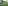
\includegraphics[width=.003\textwidth]{results_texture/1/6x8_output.png}
  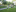
\includegraphics[width=.006\textwidth]{results_texture/1/12x16_output.png}
  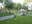
\includegraphics[width=.0125\textwidth]{results_texture/1/24x32_output.png}
  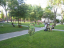
\includegraphics[width=.025\textwidth]{results_texture/1/48x64_output.png}
  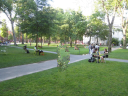
\includegraphics[width=.05\textwidth]{results_texture/1/96x128_output.png}
  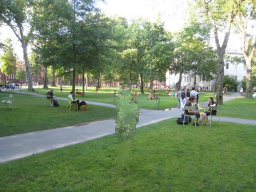
\includegraphics[width=.1\textwidth]{results_texture/1/192x256_output.png}
  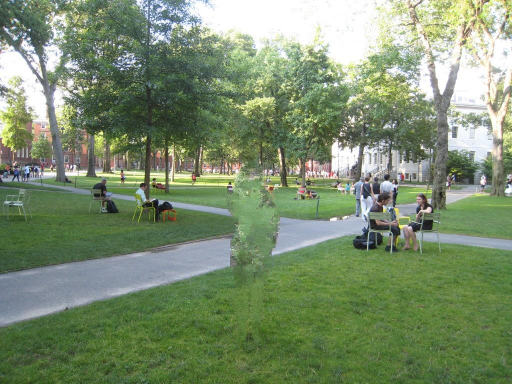
\includegraphics[width=.2\textwidth]{results_texture/1/384x512_output.png}
  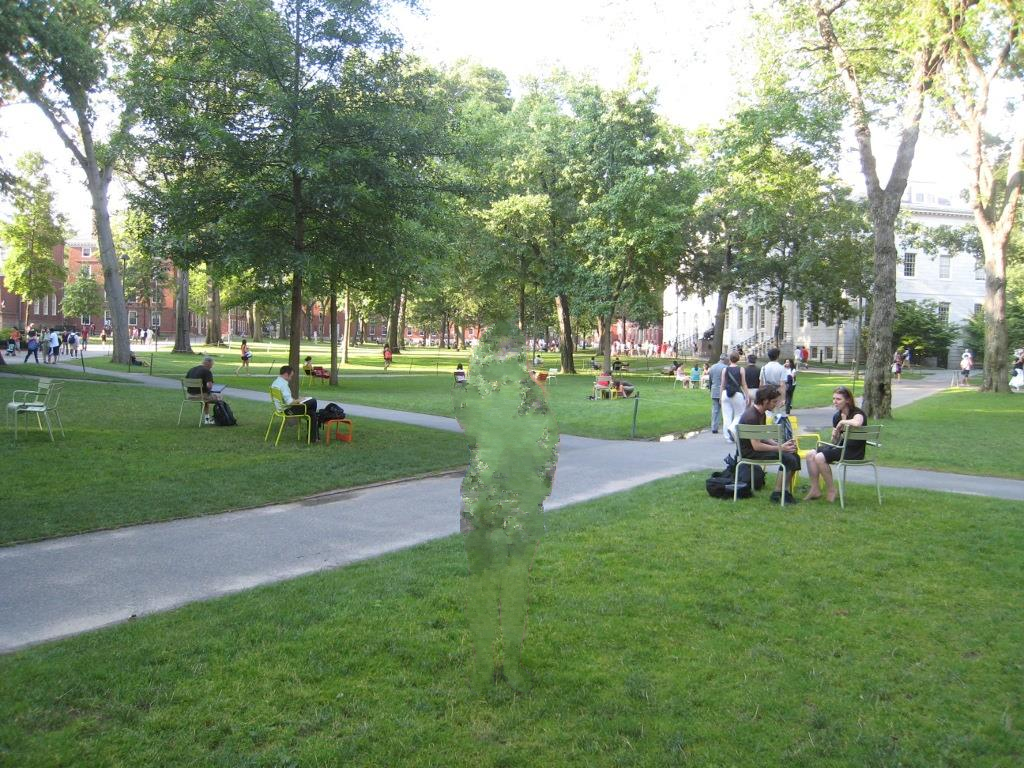
\includegraphics[width=.4\textwidth]{results_texture/1/768x1024_output.png}
  \end{center}
  
  \medskip We can notice that the texture generated doesn't exactly match the expectation we had. In order to generate a good texture, we provide the algorithm a "hint". Then we use KMeans clustering to build a partition of the pixels in clusters of textures. We restrict the nearest neighbor search to the pixels of a cluster.
  
  \begin{center}
  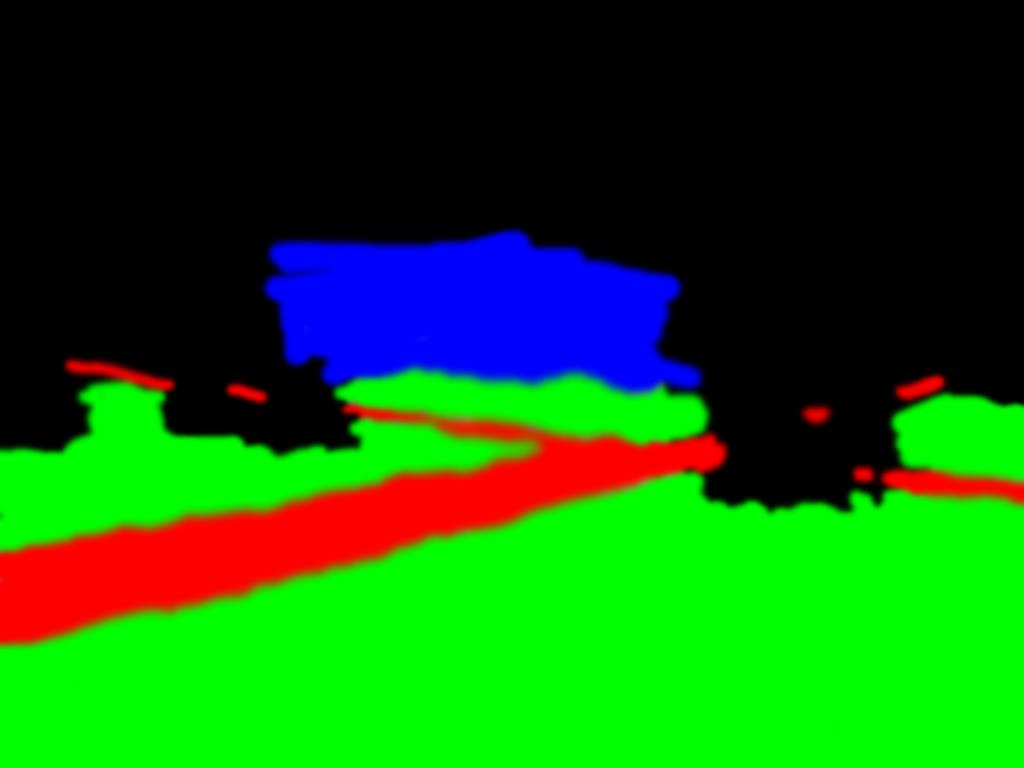
\includegraphics[width=.4\textwidth]{results_texture/2/768x1024_hint.png}
  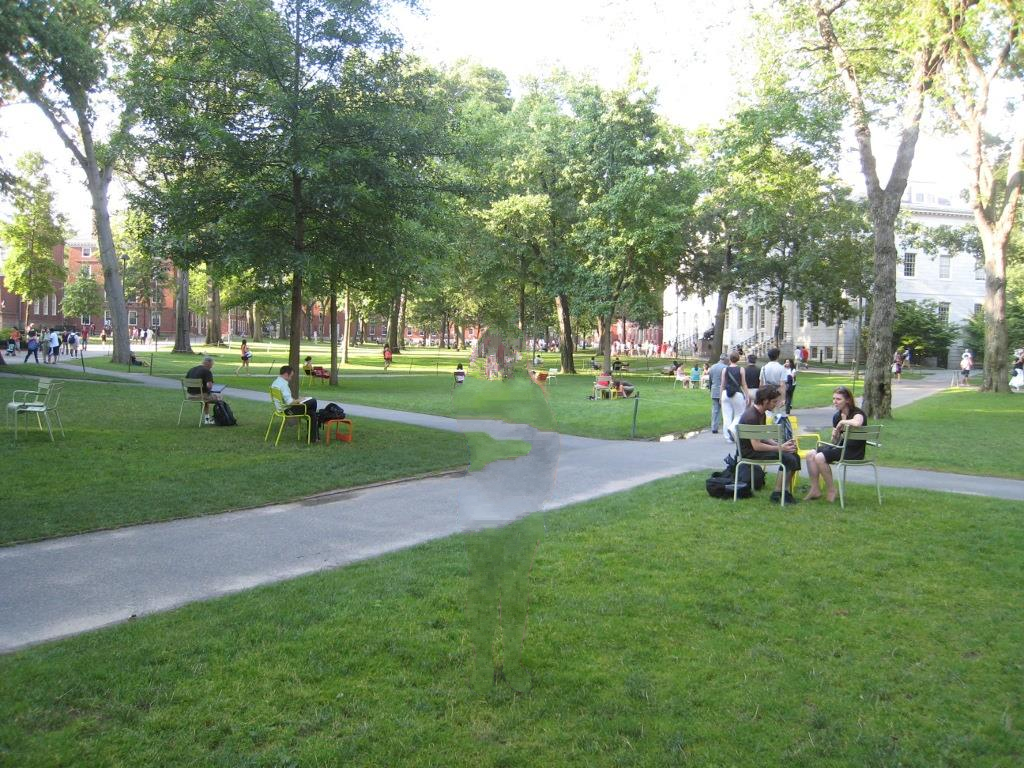
\includegraphics[width=.4\textwidth]{results_texture/2/768x1024_output.png}
  \end{center}
  
  \newpage
  
  \section{Project: Seam Carving}
  
  Reducing the size of an image can be done in several ways (resize, crop, ...). But an important part of the image can be either removed of distorded. The goal of seam carving is to detect "important" patterns, and preserve them when removing pixels from the image.
  
  \medskip The method we describe has been introduced by Avidan and Shamir in an article named "Seam carving for content-aware image resizing", published in ACM Transactions on graphics, 2007.
  
  \subsection{Description of the algorithm}
  
  The main idea is that important part of an image have a lot of details. Therefore, if we use an edge detector (\textit{e.g.} norm of the gradient of the value of pixels), we can quantify how much it would "cost" to remove one pixel from the image.
  
  To remove one column from the image, without shifting to much the rest, we can decide to delete a "continuous" path from the top-most to the lowest row. The path minimizing the total cost can be computing using dynamic programming.
  
  Once we remove one row, we can start over and remove an other one.
  
  \subsection{Implementation}
  
  I implemented the algorithm above in Python. In order to speed up the running time, I decided to keep the cost function from one iteration to one other, and setting the cost of already deleted pixels to $+\infty$ to avoid deleting them twice.
  
  \begin{center}
  \begin{tabular}{cccc}
  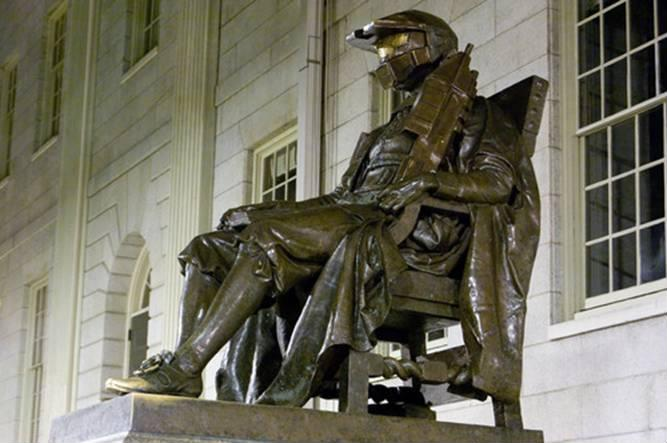
\includegraphics[height=2.5cm]{results_seamcarving/1/image_input.png} &
  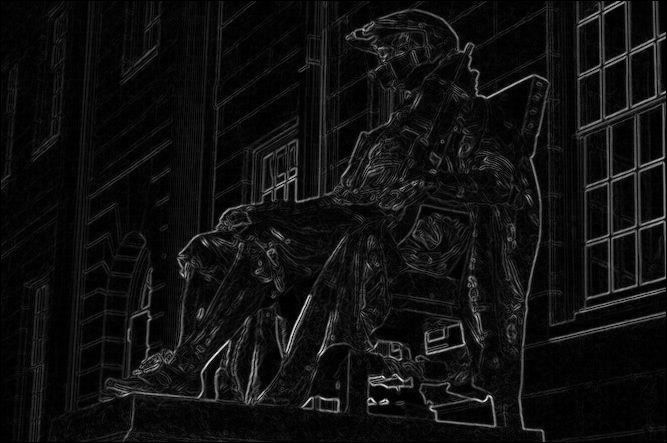
\includegraphics[height=2.5cm]{results_seamcarving/1/cost_init.png} &
  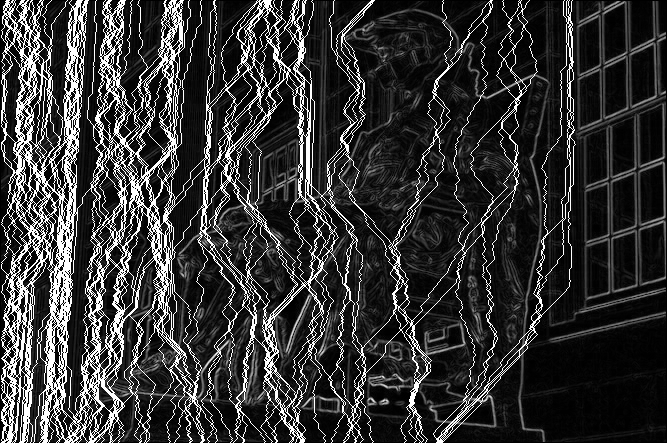
\includegraphics[height=2.5cm]{results_seamcarving/1/cost_remove.png} &
  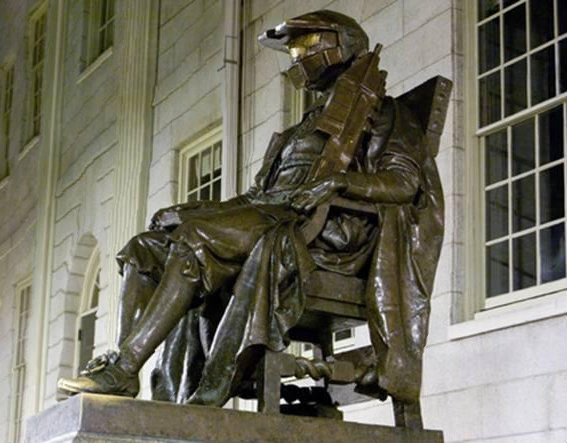
\includegraphics[height=2.5cm]{results_seamcarving/1/image_output.png} \\\\
  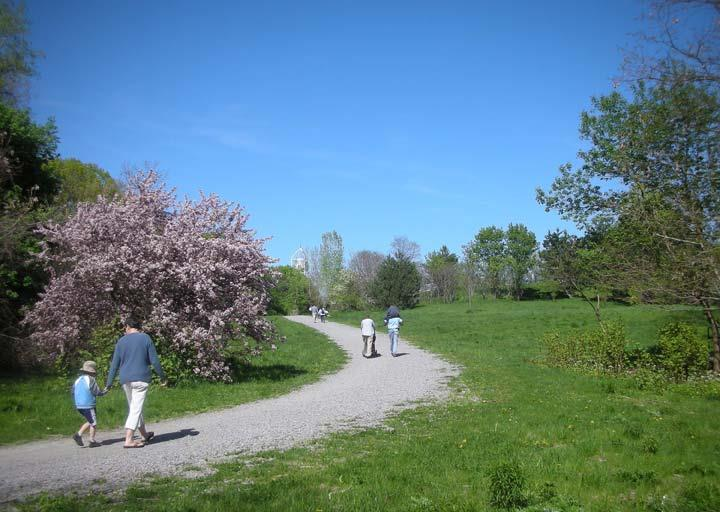
\includegraphics[height=2.7cm]{results_seamcarving/2/image_input.png} &
  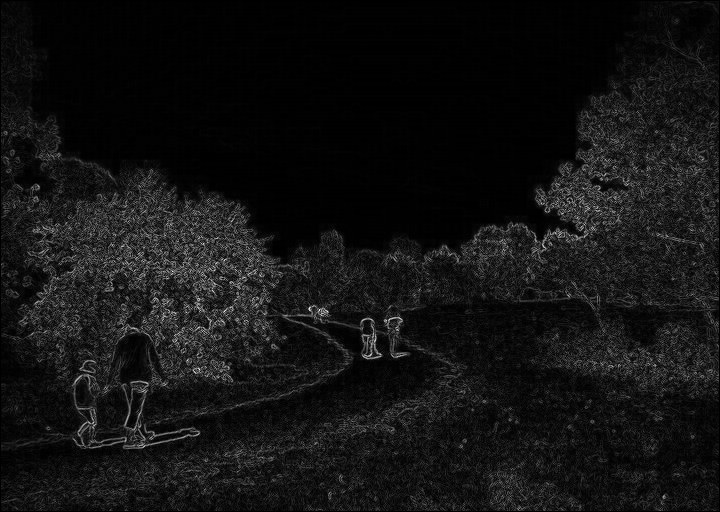
\includegraphics[height=2.7cm]{results_seamcarving/2/cost_init.png} &
  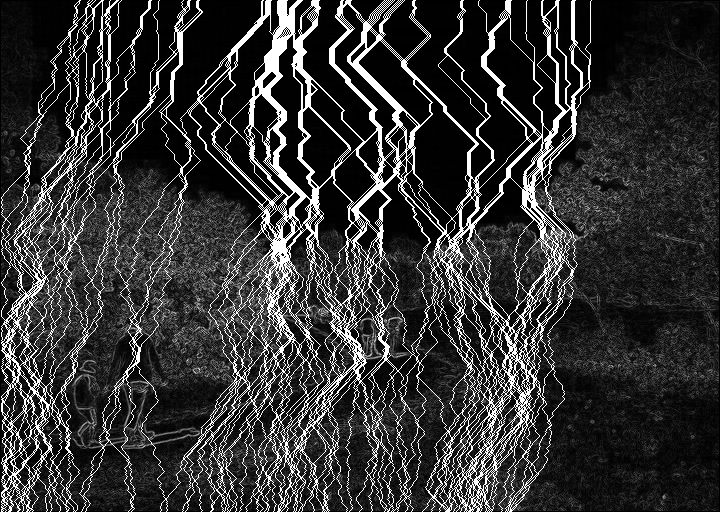
\includegraphics[height=2.7cm]{results_seamcarving/2/cost_remove.png} &
  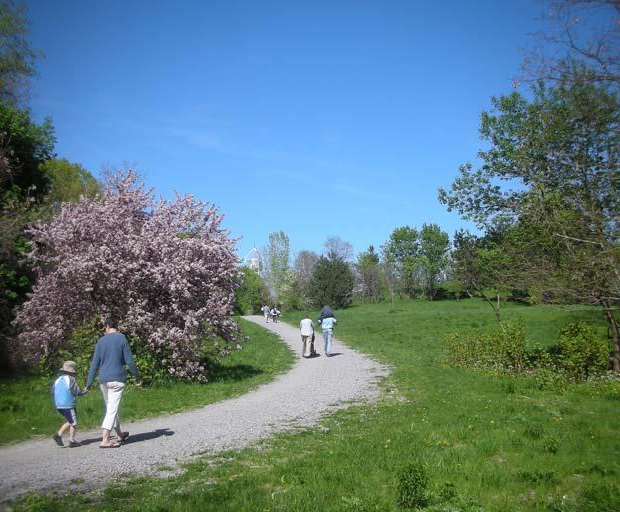
\includegraphics[height=2.7cm]{results_seamcarving/2/image_output.png} \\\\
  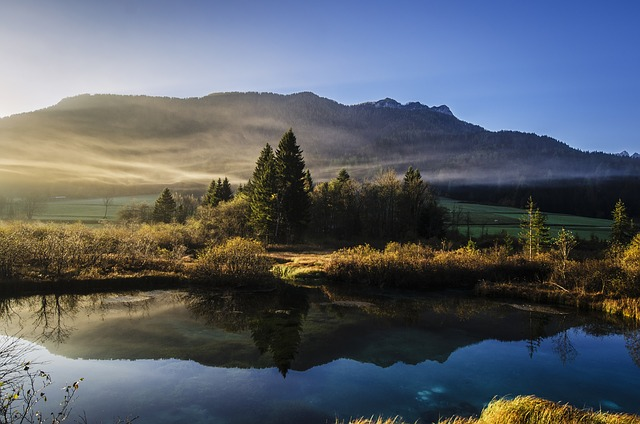
\includegraphics[height=2.5cm]{results_seamcarving/3/image_input.png} &
  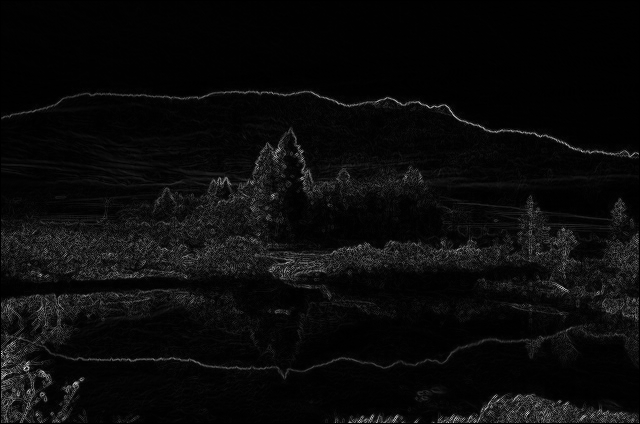
\includegraphics[height=2.5cm]{results_seamcarving/3/cost_init.png} &
  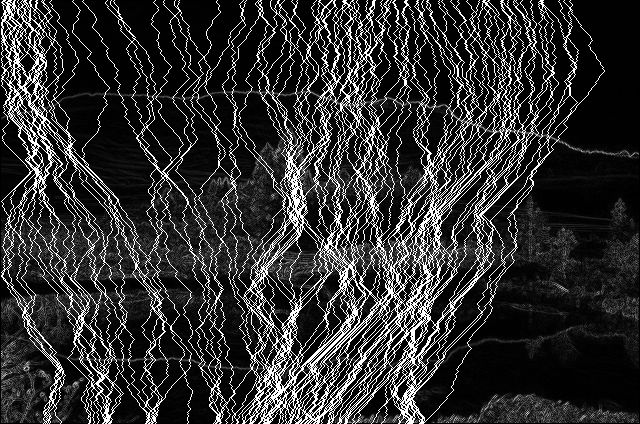
\includegraphics[height=2.5cm]{results_seamcarving/3/cost_remove.png} &
  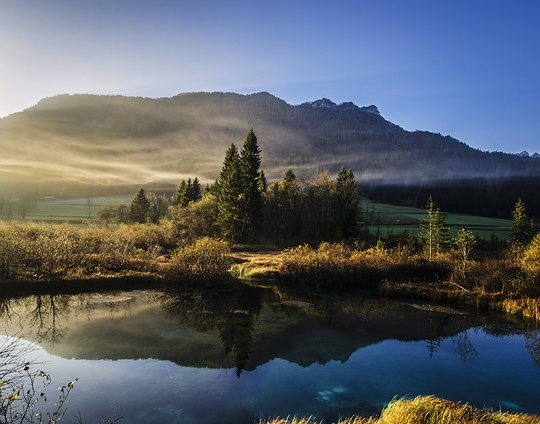
\includegraphics[height=2.5cm]{results_seamcarving/3/image_output.png}
  \end{tabular}
  \end{center}
  
\end{document}
